\section{Experimental Study}
\label{sec:study}

The empirical part of this thesis systematically investigates our implementations of the algorithms for the \WSP. In order to get an idea of the practical use of the presented algorithms, we compare them to the IP solver Gurobi\footnote{https://www.gurobi.com/}. Gurobi is a commercial solver but has free restricted licenses for academics.


\subsection{Setup}
\label{sec:study:setup}

Our experiments are conducted on random graphs of different classes. The vertices and edges are randomly weighted.\medskip

To measure the performance of each algorithm, we use Pythons $timer()$ and compare average running times. Our code was executed on a 4-core Intel machine with 16 GB of main memory. Unless otherwise noted, each series consists of 100 queries.\medskip

All our algorithms were implemented in Python and we used the packages Networkx\footnote{https://networkx.github.io/} and gurobipy. Networkx contains useful classes and functions for working with graphs and gurobipy is a python wrapper to Gurobi. Our source code can be found on the CD handed in together with this thesis. All code was designed to run on one processor core only.\medskip

For some of our algorithms, data structures for rooted trees and binary trees were implemented and used. Furthermore, procedures that create random graphs of the desired class were implemented.\medskip

Networkx provides a large variety of built-in graph generators. For constructing random paths, trees and, (not necessarily connected) graphs we used some of these generators.\medskip

We describe how we constructed random series-parallel graphs with $m$ edges. We construct a decomposition tree and the corresponding series-parallel graph in the following way. We begin with $m$ leaves representing $m$ edges. Those are also the current roots of the forest. In each step, we randomly choose 2 root vertices and add a father $v$ to them. The father is a new root, while its children are no longer roots. Also, $v$ is randomly assigned a binary operation (series composition or parallel composition). We stop when there is only one root in the forest, thus making it a tree. In each step, the number of roots in the forest is reduced by one. After $m - 1$ steps we obtain a tree with $m$ leaves corresponding to a decomposition tree for a series-parallel graph with $m$ edges.\medskip

A series-parallel graph generated in this way has between $2$ (if all compositions are parallel compositions) and $m+1$ vertices (if all compositions are series compositions). On average, a series-parallel graph with $m$ edges constructed as described above has $n = 2m-\frac{3}{2}(m-1)$ vertices. Consequently, we generate series-parallel graphs with $n$ nodes by generating series-parallel graphs with a random number of edges $m > n - 1$ until the number of desired nodes is achieved. The probability distribution over $m$ is chosen in such a way that the expected number of edges is $2n - 3$.\medskip

The construction of random connected graphs with $n$ nodes and $m$ edges, where $n-1 \leq m \leq n \cdot (n - 1)$, is done as follows: The general idea is to generate a (uniformly chosen) random spanning tree with $n$ nodes and $n - 1$ edges. Until the requested number of edges has been reached, we add an edge between any two random nodes to obtain a connected graph. Constructing a uniform spanning tree is done by generating a random walk. We create two partitions, $S$ and $T$. Initially we store all nodes in $S$. We then pick a random node from $S$, remove it and mark it as visited by putting it in $T$. In each step, we randomly pick the next node from the neighbors of the current node. If the new node is not in $T$,  meaning it has not been visited, we add an edge from the current to the new node. We set the new node as the current node and repeat. We stop when $S$ is empty. In each step of the loop, one edge is added to an unvisited node and thus not creating a cycle, while the number of elements in $S$ is reduced by one. Since we chose and removed a random node from $S$ before the loop, after $n - 1$ steps we obtain a spanning tree with $n$ nodes and $n - 1$ edges. Finally, we add random edges until the number of desired edges is reached.\medskip

We did not experience any performance differences between minimizing and maximizing the objective value. Therefore we will focus on maximizing the objective value for the remainder of this chapter. For the sake of consistency, all node and edge weights are integers between $-10$ and $10$ chosen uniformly at random. The unit of the running times we measured is seconds.\medskip

\subsection{Improvement of the IP Formulation}
\label{sec:study:ips}

As we described in Chapter \ref{sec:integer} several IP formulations for the \WSP\ and the \WISP\ were implemented. For solving IPs, the IP solver Gurobi was used. This section compares the performance and computation times of these implementations.\medskip

The graph instances used are randomly generated connected graphs as described above. To that end, the number of edges $m$ was chosen between $n - 1$ and $n \cdot (n - 1)$ uniformly at random.

\begin{table}[H]
	\centering
	\small
	\begin{tabular}{|l|l|l|l|l|l|}
		\hline
		n&IP \ref{opt:wsp}&IP \ref{opt:wsproot}&IP \ref{opt:wspflow}&IP \ref{opt:wspflowroot}&IP \href{sec:integer:seperation}{SEP}\\ \hline
		5& 0.015507& 0.005125& 0.013143& 0.003008& 0.002361\\ \hline
		10& 0.640264& 0.265688& 0.048111& 0.004004& 0.002554\\ \hline
		11& 1.796731& 0.862912& 0.059632& 0.007191& 0.003175\\ \hline
		12& 4.055318& 1.776218& 0.059833& 0.008838& 0.004095\\ \hline
		13& 10.146821& 4.451217& 0.075073& 0.013947& 0.004207\\ \hline
		14& 24.090539& 9.247563& 0.078361& 0.014200& 0.005257\\ \hline
		15& 60.995379& 22.514286& 0.104218& 0.014576& 0.008065\\ \hline
		20& -& -&0.172314& 0.025817& 0.041567\\ \hline
		30& -& -&0.449542& 0.057043& 0.050377\\ \hline
		40& -& -&0.746555& 0.102363& 2.675402\\ \hline
		50& -& -&1.031724& 0.221115& 4.249537\\ \hline
		60& -& -&1.499296& 0.231455& 10.940920\\ \hline
	\end{tabular}
	\caption{Computational performance on random instances of the IP formulations.}
	\label{table:wspips}
\end{table}

As we can see in table \ref{table:wspips}, both non-optimized IPs, namely IP \ref{opt:wsp} and IP \ref{opt:wsproot}, which have exponential many constraints cannot compete with the other IP formulations. Already for graphs with $10$ vertices, they are significantly slower than IP \ref{opt:wspflow} and IP \ref{opt:wspflowroot}. For graphs with more than $15$ vertices, it was not uncommon to experience ``out of memory'' errors. Hence, we were not able to measure the performance of IP \ref{opt:wsp} and IP \ref{opt:wsproot} for graphs with more than $15$ vertices. Both flow formulations, the rooted variant IP \ref{opt:wspflow} and the unrooted variant IP \ref{opt:wspflowroot} were able to beat all other IP formulations, especially on larger graphs. The rooted version is slower by a factor of more than $10$ which is probably due to the setup time because it has to construct and solve $n$ IPs (one for each node in the graph). IP \href{sec:integer:seperation}{SEP} started out being faster than both flow formulations, probably because it only needed a few iterations and thus the setup time was very low. But as the graphs get larger, a lot more iterations are needed and the computation time increased drastically. For graphs with $60$ vertices, it was slower than both flow formulations by a factor of more than $6$.\medskip

Figure \ref{graph:wspips} illustrates the running times of all algorithms using a logarithmic scale for the time needed.

\begin{figure}[H]
	\centering
	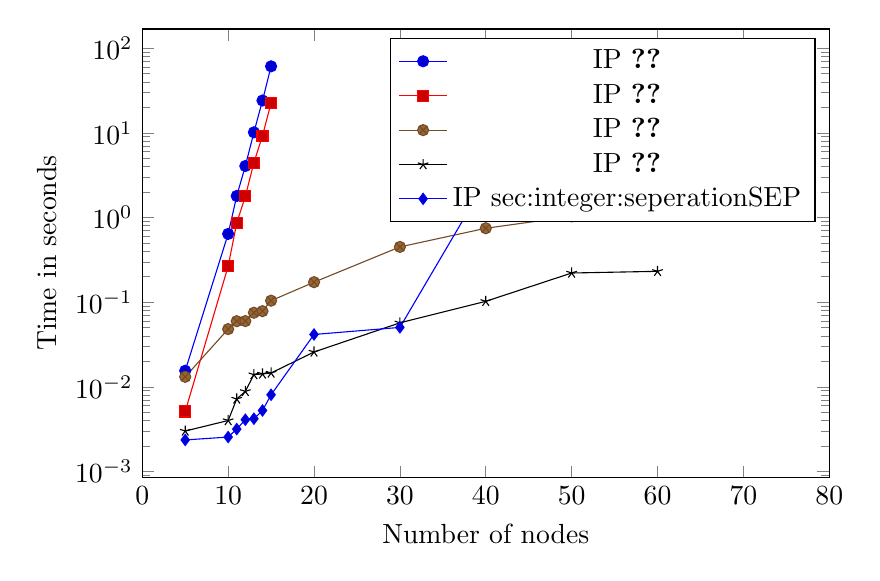
\begin{tikzpicture}
		\begin{semilogyaxis}[
			xlabel=Number of nodes,
			ylabel=Time in seconds,
			height = .6\linewidth,
			width = .85\linewidth,
			xmin=0, xmax=80]
			\addplot coordinates {
				(5,  0.015507)
				(10, 0.640264)%, 0.265688, 0.048111, 0.004004, 0.002554)
				(11, 1.796731)%, 0.862912, 0.059632, 0.008831, 0.022175)
				(12, 4.055318)%, 1.776218, 0.059833, 0.006666, 0.004095)
				(13, 10.146821)%, 4.451217, 0.075073, 0.005947, 0.004207)
				(14, 24.090539)%, 9.247563, 0.078361, 0.007731, 0.005257)
				(15, 60.995379)%, 22.514286, 0.104218, 0.009189, 0.008065)
				%(20, -, -,0.172314, 0.010840, 0.041567)
				%(30, -, -,0.449542, 0.018634, 0.050377)
				%(40, -, -,0.746555, 0.049627, 4.675402)
				%(50, -, -,1.031724, 0.036261, 2.249537)
				%(60, -, -,1.499296, 0.079477, 10.940920)
			};
			\addlegendentry{IP \ref{opt:wsp}}
			
			\addplot coordinates {
				(5,  0.005125)
				(10, 0.265688)
				(11, 0.862912)
				(12, 1.776218)
				(13, 4.451217)
				(14, 9.247563)
				(15, 22.514286)
			};
			\addlegendentry{IP \ref{opt:wsproot}}
			
			\addplot coordinates {
				(5,  0.013143)
				(10, 0.048111)
				(11, 0.059632)
				(12, 0.059833)
				(13, 0.075073)
				(14, 0.078361)
				(15, 0.104218)
				(20, 0.172314)
				(30, 0.449542)
				(40, 0.746555)
				(50, 1.031724)
				(60, 1.499296)
			};
			\addlegendentry{IP \ref{opt:wspflow}}
			
			\addplot coordinates {
				(5,  0.003008)
				(10, 0.004004)
				(11, 0.007191)
				(12, 0.008838)
				(13, 0.013947)
				(14, 0.014200)
				(15, 0.014576)
				(20, 0.025817)
				(30, 0.057043)
				(40, 0.102363)
				(50, 0.221115)
				(60, 0.231455)
			};
			\addlegendentry{IP \ref{opt:wspflowroot}}
			
			\addplot coordinates {
				(5,  0.002361)
				(10, 0.002554)
				(11, 0.003175)
				(12, 0.004095)
				(13, 0.004207)
				(14, 0.005257)
				(15, 0.008065)
				(20, 0.041567)
				(30, 0.050377)
				(40, 2.675402)
				(50, 4.249537)
				(60, 10.940920)
			};
			\addlegendentry{IP \href{sec:integer:seperation}{SEP}}
		\end{semilogyaxis}
	\end{tikzpicture}
	\caption{Illustration of the computation times of the IP formulations.}
	\label{graph:wspips}
\end{figure}

For the remainder of this chapter, we mainly use IP \ref{opt:wspflowroot} for measuring the performance of solving the \WSP\ using Gurobi. Also, we noticed that graph density seems to have a big impact on the running time of all IP formulations. Since that impact was percentage-wise the same for all IP formulations, we did not consider it for this segment.\medskip


\subsection{Performance of the Dynamic Program}
\label{sec:study:dynprog}

In the last section, we have seen that the flow formulation (see IP \ref{opt:wspflowroot}) was the most efficient way of solving the \WSP\ using Gurobi. In this section, the performance of the dynamic program from section \ref{sec:wsp} is compared to the performance of Gurobi.\medskip

We implemented the dynamic program from Chapter \ref{sec:dynamicprog} for paths, trees, and series-parallel graphs. To compare the performance of the implementations we randomly generated graphs of those classes with different sizes. The size of a graph is given by the number of nodes in the graph.\medskip

In Table \ref{table:wspdyn} average running times of the algorithms on paths, trees, and series-parallel graphs are shown.

\begin{table}[H]
	\centering
	\resizebox{\textwidth}{!}{%
		\begin{tabular}{|l|l|l|l|l|l|l|}
			\hline
			&\multicolumn{2}{c|}{paths}&\multicolumn{2}{c|}{trees}&\multicolumn{2}{c|}{series-parallel graphs}\\ \hline
			n&dynamic prog&IP \ref{opt:wspflowroot}&dynamic prog&IP \ref{opt:wspflowroot}&dynamic prog&IP \ref{opt:wspflowroot}\\ \hline
			10&0.000106&0.013639&0.000194&0.005969&0.000656&0.008037\\ \hline
			20&0.000160&0.034162&0.000386&0.024114&0.001478&0.056467\\ \hline
			30&0.000220&0.120945&0.000662&0.086717&0.002345&0.070305\\ \hline
			40&0.000270&0.340605&0.000886&0.138077&0.003098&0.152056\\ \hline
			50&0.000322&0.863015&0.001063&0.316319&0.003952&0.230241\\ \hline
			60&0.000376&2.099835&0.001363&0.990999&0.004976&1.349487\\ \hline
			75&0.000603&11.706951&0.001930&1.576299&0.006210&4.346551\\ \hline
			100&0.000627&28.071109&0.002127&4.881766&0.008490&10.715087\\ \hline
		\end{tabular}
	}%
	\caption{Computational performance of the dynamic program on random paths, trees and series-parallel graphs.}
	\label{table:wspdyn}
\end{table}

As we can see in Table \ref{table:wspdyn} our procedure is significantly faster than Gurobi on all instances. By increasing the number of vertices in the graph, the dynamic program really shows its power. Already for graphs with $30$ or fewer vertices, significant differences in computation times can be seen. For a graph with $100$ vertices, the computation time is faster by a factor of more than $2000$. For paths and series-parallel graphs this factor is even larger.\medskip

In the next series, we wanted to examine the influence of graph density on the performance of the dynamic program. For this, we generated random series-parallel graphs with $m$ edges until the desired number of vertices $n$ was achieved.

\begin{table}[H]
	\centering
	\small
	\begin{minipage}{.5\linewidth}
		\centering
		\begin{tabular}{|l|l|l|l|}
			\hline
			n&m&dynamic prog&IP \ref{opt:wspflowroot}\\ \hline
			50&50&0.002479&0.629711\\ \hline
			50&75&0.003967&0.102970\\ \hline
			50&100&0.005365&0.061309\\ \hline
			50&250&0.014865&0.134188\\ \hline
			50&500&0.028244&1.047685\\ \hline
			50&1000&0.063950&13.621358\\ \hline
%			50&50&0.002619&1.147671\\ \hline
%			50&75&0.003737&1.022072\\ \hline
%			50&100&0.005037&0.362395\\ \hline
%			50&250&0.018587&0.617618\\ \hline
%			50&500&0.028353&0.937060\\ \hline
%			50&1000&0.064335&3.446711\\ \hline
		\end{tabular}
	\end{minipage}%
	\begin{minipage}{.5\linewidth}
		\centering
		\begin{tabular}{|l|l|l|l|}
			\hline
			n&m&dynamic prog&IP \ref{opt:wspflowroot}\\ \hline
			100&100&0.005209&5.852813\\ \hline
			100&250&0.014053&0.250138\\ \hline
			100&500&0.027513&0.616554\\ \hline
			100&1000&0.067332&26.753307\\ \hline
		\end{tabular}
	\end{minipage}%
	\caption{Impact of graph density on the computational performance.}
	\label{table:density}
\end{table}

Turns out, that density has a linear impact on the performance of the dynamic program which was to be expected since its theoretical running time is $\OO(m)$. In Table \ref{table:density} we can see that the running time seems to double every time the number of edges is doubled. In all cases, the dynamic program is faster than Gurobi. For rather sparse and dense graphs this gap becomes larger. For a graph with $50$ vertices and $1000$ edges the dynamic program is faster than Guribi by a factor of more than $200$.

\subsection{Polyhedral Results}
\label{sec:study:poly}

In this section, we compare the proposed IP formulations practically with respect to their quality of LP bounds. In the following, let $\PP_{LP}(\cdot)$ denote the polytopes of the LP-relaxations of the IP models presented in section \ref{sec:integer} and $\textsc{opt}_{LP}(\cdot)$ their optimal LP-values. Moreover, let $\textsc{opt}_{IP}$ denote the objective value of the IP.\medskip

We generated random connected graphs with $n$ nodes. Hereby, the number of edges $m$ was chosen between $n - 1$ and $n \cdot (n - 1)$ uniformly at random. In Table \ref{table:relaxation} the objective value and the gap (as percentages) of each instance is shown:

\begin{table}[H]
	\centering
	\resizebox{\textwidth}{!}{%
		\begin{tabular}{|l|l|l|l|l|l|l|}
			\hline
			&\multicolumn{2}{c|}{LP \ref{opt:wsproot}} &\multicolumn{2}{c|}{LP \ref{opt:wsp}} &\multicolumn{2}{c|}{LP \ref{opt:wspflowroot}}\\ \hline
			$\textsc{opt}_{IP}$ & $\textsc{opt}_{LP}\cut$ & gap [\%] & $\textsc{opt}_{LP}\cutr$ & gap [\%] & $\textsc{opt}_{LP}\flow$ & gap [\%] \\ \hline
			24&24.50&2.04&27.59&13.00&29.00&17.24\\ \hline 
			29&29.00&0.00&29.00&0.00&29.00&0.00\\ \hline 
			14&17.50&20.00&22.11&36.68&29.00&51.72\\ \hline 
			29&29.50&1.69&30.86&6.01&31.50&7.94\\ \hline 
			33&33.50&1.49&33.90&2.65&34.00&2.94\\ \hline 
			31&31.50&1.59&31.89&2.79&32.00&3.12\\ \hline 
			12&12.00&0.00&12.50&4.00&13.00&7.69\\ \hline 
			23&23.00&0.00&23.00&0.00&23.00&0.00\\ \hline 
			22&30.00&26.67&36.11&39.08&41.00&46.34\\ \hline 
			54&55.50&2.70&55.50&2.70&55.50&2.70\\ \hline 
			16&16.00&0.00&16.77&4.59&18.00&11.11\\ \hline 
			47&47.00&0.00&47.00&0.00&47.00&0.00\\ \hline 
			40&40.00&0.00&40.00&0.00&40.00&0.00\\ \hline 
			56&57.50&2.61&65.57&14.59&68.00&17.65\\ \hline 
			47&47.00&0.00&47.00&0.00&47.00&0.00\\ \hline 
		\end{tabular}
	}%
	\caption{Gaps [\%] reached by the LP relaxations.}
	\label{table:relaxation}
\end{table}

In Table \ref{table:relaxation} we report the results obtained for the LP relaxations. The gap between the optimal objective value and the LP bound varies greatly between $0$ and more than $50$ percent. Both heuristics were able to obtain the optimal objective value for some instances. In general, $\textsc{opt}_{LP}\cut$ reaches the smallest gaps with an average of $3.91$ percent, the maximal gap being $26.67$ percent. It is followed by $\textsc{opt}_{LP}\cutr$ with an average of $8.40$ percent, and a maximum of $39.08$ percent. Finally $\textsc{opt}_{LP}\flow$ reaches an average gap of $11.23$ percent and a maximal gap of $51.72$ percent.\medskip

For all instances, we can see that the objective value of the flow formulation is larger than the value of the rooted cut formulation. Furthermore, the objective value of the rooted cut formulation is larger than the value of the unrooted cut formulation. This lets us suspect that
$$\textsc{opt}_{LP}\cut \leq \textsc{opt}_{LP}\cutr \leq \textsc{opt}_{LP}\flow$$
which also gives the impression that
$$\PP_{LP}\cut \subseteq \PP_{LP}\cutr \subseteq \PP_{LP}\flow.$$

\subsection{Preprocessing}
\label{sec:study:preprocess}

We continue by investigating whether the preprocessing scheme from section \ref{sec:approximation:preprocess} yields a noticeable benefit. How big is the reduced instance compared to the original instance? How large is the performance boost when using the preprocessing scheme, if any?\medskip

For this segment, we generated random connected graphs (with parallel edges) as described in Section \ref{sec:study:setup}. The following table \ref{table:preprocesssize} enlists the sizes of the original instances compared to the average sizes of the reduced instances.

\begin{table}[H]
	\centering
	\small
	\begin{minipage}{.5\linewidth}
		\centering
		\begin{tabular}{|l|l|l|l|}
			\hline
			\multicolumn{2}{|c|}{Original instance}&\multicolumn{2}{c|}{Reduced instance}\\ \hline
			n& m& n& m\\ \hline
			10&20&2.28&1.28\\ \hline
			10&30&4.74&4.43\\ \hline
			10&40&2.93&1.54\\ \hline
			50&100&15.35&22.80\\ \hline
			50&150&7.90&6.13\\ \hline
			50&200&2.21&1.61\\ \hline
			75&150&20.00&36.34\\ \hline
			75&225&7.12&6.43\\ \hline
			75&300&4.09&3.65\\ \hline
		\end{tabular}
	\end{minipage}%
	\begin{minipage}{.5\linewidth}
		\centering
		\begin{tabular}{|l|l|l|l|}
			\hline
			\multicolumn{2}{|c|}{Original instance}&\multicolumn{2}{c|}{Reduced instance}\\ \hline
			n& m& n& m\\ \hline
			100&200&29.22&42.17\\ \hline
			100&300&12.92&15.76\\ \hline
			100&400&9.64&8.11\\ \hline
			250&500&70.05&103.38\\ \hline
			250&750&37.89&46.32\\ \hline
			250&1000&14.90&16.75\\ \hline
			500&1000&150.91&249.41\\ \hline
			500&1500&57.14&75.07\\ \hline
			500&2000&25.18&32.69\\ \hline
		\end{tabular}
	\end{minipage} 
	\caption{Average graph size of reduced instance obtained by applying the preprocessing scheme from section \ref{sec:approximation:preprocess} compared to the original graph size.}
	\label{table:preprocesssize}
\end{table}

Of course, these results depend on the weights in the graph. Table \ref{table:preprocesssize} shows that there is a correlation between the size of the reduced instance and the density of the original instance. The denser the input graph is, the smaller the reduced graph will be. This is probably caused by the fact, that weights on vertices and edges use the same weight distribution. Also, the number of parallel edges in the graph is higher which is utilized by the preprocessing procedure. In general, graphs are reduced by at least $50$ percent for all instances that we tested.\medskip

For the performance measurement, we solved an instance as follows. First, we solved the instance to optimality and measured the time needed. Then we applied the preprocessing scheme to the same graph and solved the reduced instance. The time measured includes the preprocessing scheme as well as the time needed to solve the reduced instance. For computing a solution IP \eqref{opt:wspflowroot} was used. Table \ref{table:preprocess} shows the computations times for both cases.

\begin{table}[H]
	\centering
	\small
	\begin{tabular}{|l|l|l|l|}
		\hline
		n&m&with preprocessing&without preprocessing\\ \hline
		10&20&0.004879&0.005269\\ \hline
		10&30&0.006946&0.007743\\ \hline
		10&40&0.007620&0.010667\\ \hline
		50&100&0.051437&0.060431\\ \hline
		50&150&0.045415&0.047085\\ \hline
		50&200&0.057990&0.066576\\ \hline
		100&200&0.185324&0.202422\\ \hline
		100&300&0.102997&0.115853\\ \hline
		100&400&0.150227&0.186277\\ \hline			
		250&500&1.330858&1.456818\\ \hline
		250&750&0.495078&0.508311\\ \hline
		250&1000&0.942581&1.025909\\ \hline
		500&1000&4.531664&5.518316\\ \hline
		500&1500&2.875006&2.007461\\ \hline
		500&2000&3.938611&4.455854\\ \hline
	\end{tabular}
	\caption{Computational performance when using the preprocessing scheme from section \ref{sec:approximation:preprocess}.}
	\label{table:preprocess}
\end{table}

In Table \ref{table:preprocess} we observe that on average, using the preprocessing scheme yields a noticeable performance boost. As the instances get larger, the decrease in computation time is more substantial. For graphs with $100$ vertices or less the difference is not very large. But for graphs with $500$, vertices the speedup in computation time is almost 1 second. In general, using the preprocessing procedure seems to decrease the running time by almost $10$ percent.


\subsection{Heuristics}
\label{sec:study:heuristic}

Continuing, we would like to compare the proposed heuristic algorithms and the quality of their solutions. In the following, let $\textsc{heu}_{NS}$ denote Procedure \ref{proc:wspnodes} and $\textsc{heu}_{ST}$ the procedure from section \ref{sec:approximation:spanningtree}.\medskip

First, let us start with the computational performance of the heuristic solutions. For this test randomly generated connected graphs with $n$ nodes were used. As previously, the number of edges $m$ was chosen between $n - 1$ and $n \cdot (n - 1)$ uniformly at random. For $\textsc{heu}_{NS}$ we used IP \ref{opt:wspflowroot} to solve the modified version of \textsc{wsp} (see step 4 in Procedure \ref{proc:wspnodes}). From the results above we conduct that IP \ref{opt:wspflowroot} can be efficiently solved for graphs with $100$ vertices. Thus, we set $N \defeq 100$ as an upper bound of the number of nodes for the modified instance.

\begin{table}[H]
	\centering
	\small
	\begin{tabular}{|l|l|l|l|}
		\hline
		n&IP \ref{opt:wspflowroot}&$\textsc{heu}_{NS}$&$\textsc{heu}_{ST}$\\ \hline
		10&0.008435&0.003538&0.000870\\ \hline
		25&0.024684&0.012868&0.002372\\ \hline
		50&0.047114&0.075030&0.004126\\ \hline
		100&0.204004&0.393630&0.010188\\ \hline
		250&0.964690&4.934293&0.035741\\ \hline
		500&6.725403&36.911216&0.107158\\ \hline
		1000&81.908922&297.658889&0.427159\\ \hline		
	\end{tabular}
	\caption{Computational performance of the heuristic procedures compared to IP \eqref{opt:wspflowroot}.}
	\label{table:heuristictime}
\end{table}

Table \ref{table:heuristictime} presents the running times of Gurobi using the flow formulation \eqref{opt:wspflowroot} and of both heuristic methods $\textsc{heu}_{NS}$ and $\textsc{heu}_{ST}$. The node set heuristic presented in section \ref{sec:approximation:nodeset} cannot compete with Gurobi. Already for graphs with $250$ vertices, significant differences in computation times can be seen. This is caused by a large number of inequalities in the modified instance of the problem. We fixed a set of the nodes to be in the solution. Thus, we reduced the number of nodes Gurobi has to select, but not the number of edges. This behavior gets worse if we increase the number of nodes. For a graph with $1000$ vertices, the method is worse than Gurobi by a factor of $300$. Hence, we conclude that Procedure \ref{proc:wspnodes} is not of practical relevance. In contrast, $\textsc{heu}_{ST}$ can be computed very efficiently even for large instances. For only $50$ vertices the difference is the procedure from section \ref{sec:approximation:spanningtree} is faster than Gurobi by a factor of $10$. For $500$ vertices the factor has already increased to $60$ and for $1000$ vertices the procedure is faster by a factor of $200$.\medskip

Now we want to regard the solution quality of $\textsc{heu}_{NS}$ and $\textsc{heu}_{ST}$. For each heuristic Table \ref{table:heuristicquality} shows the minimal, maximal, and average gap reached within $100$ iterations.

\begin{table}[H]
	\centering
	\small
	\begin{tabular}{|l|l|l|l|}
		\hline
		&\multicolumn{3}{c|}{$\textsc{heu}_{NS}$}\\ \hline
		n&max. gap [\%]&min. gap [\%]&avg. gap [\%]\\ \hline
		10&24.44&0.00&2.69\\ \hline 
		25&16.54&0.00&2.73\\ \hline 
		50&9.51&0.00&2.68\\ \hline 
		100&9.31&0.69&3.80\\ \hline 
		250&10.10&2.36&4.99\\ \hline 
		500&7.79&4.33&6.70\\ \hline 
		1000&7.56&4.68&6.05\\ \hline 
	\end{tabular}\bigskip

	\begin{tabular}{|l|l|l|l|}
		\hline
		&\multicolumn{3}{c|}{$\textsc{heu}_{ST}$}\\ \hline
		n&max. gap [\%]&min. gap [\%]&avg. gap [\%]\\ \hline
		10&33.33&0.00&9.31\\ \hline 
		25&32.71&1.68&12.45\\ \hline 
		50&23.08&5.56&13.05\\ \hline 
		100&24.40&6.49&13.66\\ \hline 
		250&17.50&8.90&12.84\\ \hline 
		500&15.30&10.79&12.68\\ \hline 
		1000&15.23&11.46&13.31\\ \hline 
	\end{tabular}
	\caption{Minimal, maximal, and average gaps reached by the heuristic procedures on graphs of different size.}
	\label{table:heuristicquality}
\end{table}

We have seen above that the computation time of $\textsc{heu}_{NS}$ cannot compete with Gurobi. Nevertheless, Table \ref{table:heuristicquality} shows that the solution quality is impressive. Its average gap to $\textsc{opt}_{IP}$ is approximately $12.5$ percent. The maximal gap decreases from $33.33$ percent on graphs with $10$ nodes to $15.23$ percent on graphs with $1000$ nodes while the minimal gap increases from $0$ to $11.46$ percent for the instances we tested. For almost all instances $\textsc{heu}_{NS}$ obtains a better heuristic solution than $\textsc{heu}_{ST}$. Its average gap to $\textsc{opt}_{IP}$ is approximately $3$ percent. For small instances of up to $50$ vertices, the procedure from section \ref{sec:approximation:spanningtree} was able to obtain the optimal objective value. For bigger instances, the maximal gap is at most $10.10$ percent on the instances we tested, while its minimal gap increased to almost $5$ percent.\medskip

Therefore, we conclude that $\textsc{heu}_{ST}$ can be used to obtain decent heuristic solutions and lower bounds for the optimal objective value. Although $\textsc{heu}_{NS}$ reaches tighter bounds in terms of the objective value, we do not recommend using it due to its bad computation time.

